
% =====================================================================
\section{Numerical verification}
\label{sec:validation}
% =====================================================================

The results are proved from the premises and require no computation. It is
nonetheless instructive to exhibit them on concrete instances and to display the
quantitative shape of each. This section reports an exhaustive numerical witness:
every result---the derived floor, T0--T8, and the measurement theorems---is tested
on a large family of explicitly constructed finite contact graphs, and the
measured quantities are plotted against the bounds the theorems predict.

\subsection{Method}

A contact graph is realised as a finite, connected, weighted graph on a vertex
set of parts together with a distinguished \emph{medium} vertex adjacent to every
part; edge weights are drawn at or above a floor $\floorc>0$. By construction such
an instance satisfies \Cref{ax:finite}. On each instance the cuts, boundary
costs, the global minimum-cut residual, the separation of a part from the medium,
the committed count along gated walks, and the quotient cut weights are computed
directly from the definitions---by exact enumeration over subsets, so every
minimum is the true value---and each theorem's inequality, identity, or invariance
is checked. A \emph{measurement} is realised as a reshuffling: a weight-preserving
relabelling of the non-medium vertices, which conserves the total weight and the
medium and changes only the labelling.

A randomised sweep drew instances of varying part count, floor, edge density, and
weight spread, and ran all ten theorem-group checks on each, with a fixed
two-cluster construction as a standalone witness for the region-valued residual.
Across $600$ instances the suite performed $149{,}793$ individual checks, all of
which passed: no cut was sharp; every boundary, cut, residual, private invariant,
and quotient edge met the floor; the residual was invariant under every
reshuffling; the committed count was strictly monotone on every walk;
authored instances preserved the floor with all forward-closure states distinct;
and the separation of a part from the medium never reached zero under any sequence
of measurements. The figures below are drawn from these same computations.

\subsection{The derived floor and T0}

\begin{figure*}[!htbp]
    \centering
    
\includegraphics[width=\textwidth]{figures/panel_1.png}
    \caption{\textbf{Floor from Infinitude: every thing carries a positive residual.}
    (\textbf{A})~Identification residual of a thing (boundary cost of a proper
    part) on the linear $y$-axis versus the floor $\beta$ on the linear $x$-axis,
    over $\sim\!250$ instances; the red line is $y=\beta$ and every point lies on
    or above it, the content of \Cref{thm:floor-infinitude}.
    (\textbf{B})~Distribution of residual$/\beta$ on the linear $x$-axis, supported
    entirely at and above $1$ (red): no thing has sub-floor residual; the
    comparison never completes.
    (\textbf{C})~Per-instance minimum residual versus floor, on or above the
    equality line---the derived floor is strictly positive on every instance
    (\Cref{cor:floor-derived}).
    (\textbf{D})~Three-dimensional surface of the per-instance minimum residual
    over vertex count and floor; strictly positive throughout. Viewing angle:
    elevation $22^{\circ}$, azimuth $-60^{\circ}$.}
    \label{fig:panel-ground}
\end{figure*}

\begin{figure*}[!htbp]
    \centering
    
\includegraphics[width=\textwidth]{figures/panel_2.png}
    \caption{\textbf{T0, the Floor Theorem: no sharp cut.}
    (\textbf{A})~Cut weight of every realisable part on the linear $y$-axis versus
    floor $\beta$ on the linear $x$-axis; all points lie on or above $y=\beta$
    (red), confirming \Cref{thm:floor}.
    (\textbf{B})~Distribution of cut$/\beta$, supported entirely above $1$ (red):
    across all parts of all instances no cut is sharp.
    (\textbf{C})~Per-instance minimum cut versus floor, above the equality line.
    (\textbf{D})~Three-dimensional surface of the per-instance minimum cut over
    edge count and floor, strictly positive everywhere. Viewing angle: elevation
    $20^{\circ}$, azimuth $-55^{\circ}$.}
    \label{fig:panel-T0}
\end{figure*}

\subsection{Negation, residual, and the private invariant}

\begin{figure*}[!htbp]
    \centering
    
\includegraphics[width=\textwidth]{figures/panel_3.png}
    \caption{\textbf{T1, individuation by negation.}
    (\textbf{A})~Size of a part $|U|$ versus size of its complement, over all
    sampled parts; every part is fixed by its complement.
    (\textbf{B})~Distribution of the involution error
    $\lvert U\,\triangle\,\complement\complement U\rvert$, a single bar at $0$
    (red): complementation is an exact involution
    (\Cref{lem:involution}).
    (\textbf{C})~$|U|+|\complement U|$ versus $|V|$, on the diagonal: a part and
    its negation-set partition the whole exactly.
    (\textbf{D})~Three-dimensional scatter of $(|U|,|\complement U|,|V|)$ lying on
    the plane $|U|+|\complement U|=|V|$. Viewing angle: elevation $24^{\circ}$,
    azimuth $-58^{\circ}$.}
    \label{fig:panel-T1}
\end{figure*}

\begin{figure*}[!htbp]
    \centering
    
\includegraphics[width=\textwidth]{figures/panel_4.png}
    \caption{\textbf{T2/T3, the residual is a conserved region.}
    (\textbf{A})~Global minimum-cut residual versus floor, on or above the
    equality line (\Cref{thm:residual-region}).
    (\textbf{B})~Residual after a reshuffling versus before, exactly on the
    diagonal: the residual is invariant under reshuffling
    (\Cref{thm:residual-invariant}); maximum deviation at machine precision.
    (\textbf{C})~Distribution of the size of the smaller side of the minimum cut;
    mass at sizes $\ge2$ (red threshold at $1.5$) shows the residual is realised by
    multi-vertex regions, not points. The standalone two-cluster witness attains
    residual $=\beta=1$ with both sides of size $3$ ($\{0,1,2\}\mid\{3,4,5\}$): a
    region, never a point.
    (\textbf{D})~Three-dimensional surface of residual over floor and minimum-cut
    side size. Viewing angle: elevation $22^{\circ}$, azimuth $-60^{\circ}$.}
    \label{fig:panel-T2T3}
\end{figure*}

\begin{figure*}[!htbp]
    \centering
    
\includegraphics[width=\textwidth]{figures/panel_5.png}
    \caption{\textbf{T4, the private invariant of a part.}
    (\textbf{A})~Private invariant (a part's boundary cost to the medium) versus
    floor, on or above $y=\beta$ (red): positive for every part
    (\Cref{thm:private}).
    (\textbf{B})~Private invariant versus part degree: bounded below by the floor
    independently of degree.
    (\textbf{C})~Distribution of invariant$/\beta$, supported above $1$ (red).
    (\textbf{D})~Three-dimensional surface of the per-instance minimum private
    invariant over vertex count and floor, strictly positive. Viewing angle:
    elevation $22^{\circ}$, azimuth $-58^{\circ}$.}
    \label{fig:panel-T4}
\end{figure*}

\subsection{Gating, non-return, and the quotient}

\begin{figure*}[!htbp]
    \centering
    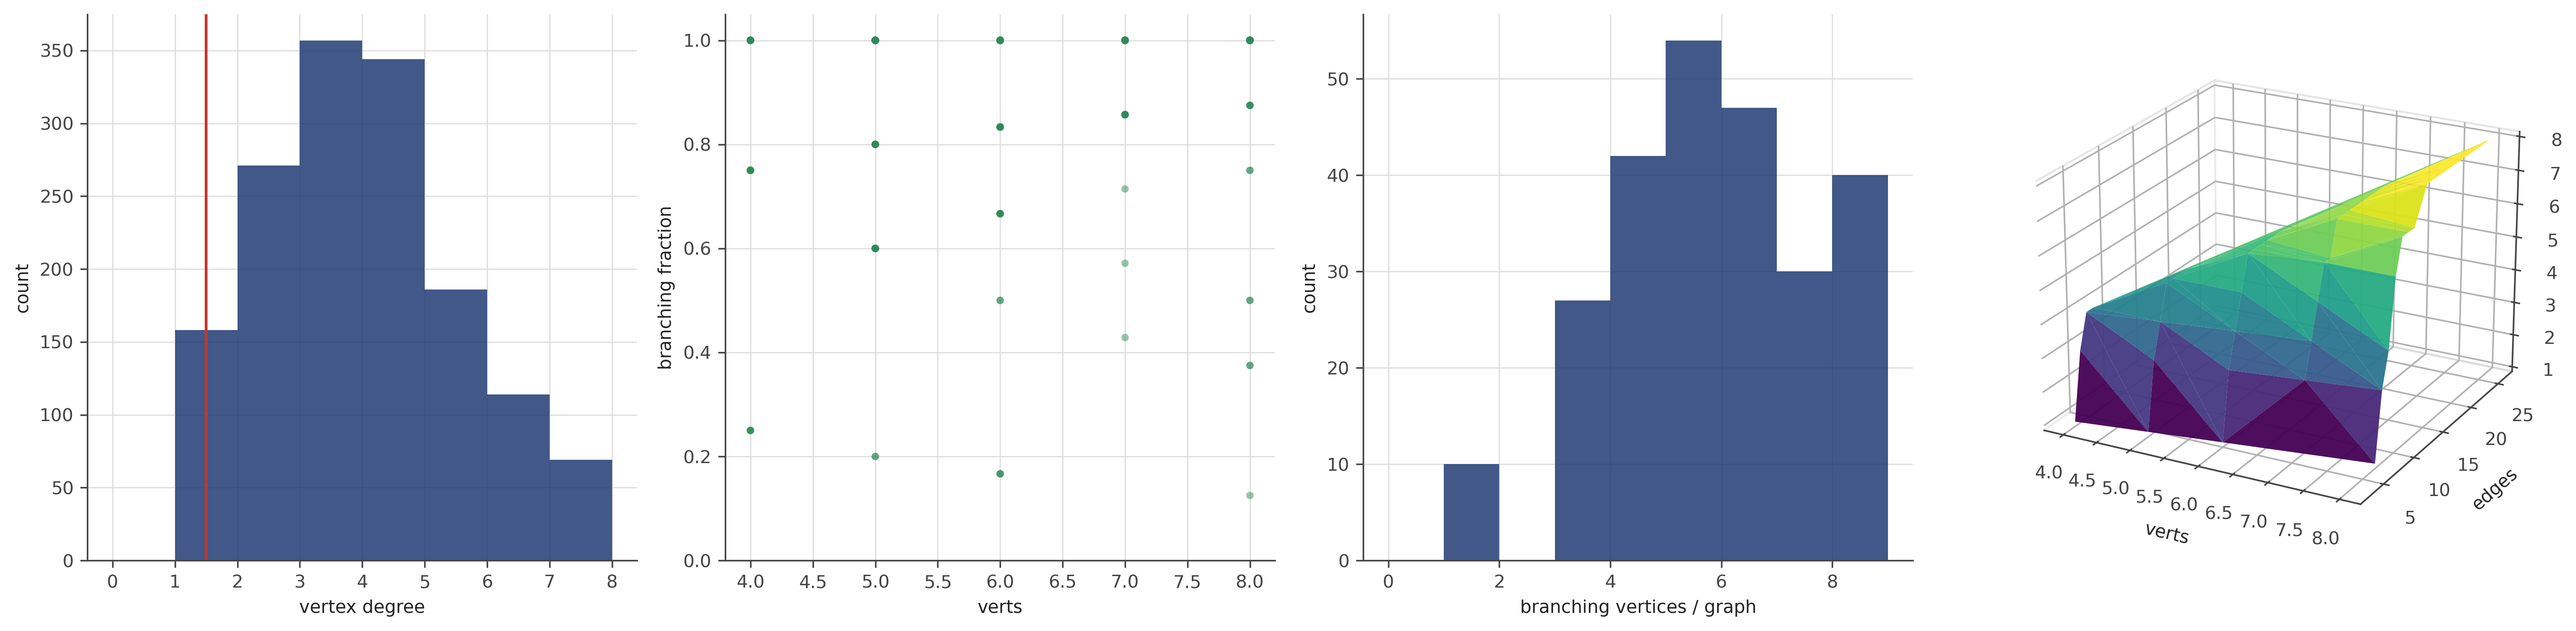
\includegraphics[width=\textwidth]{figures/panel_6.png}
    \caption{\textbf{T5, selection requires a gate.}
    (\textbf{A})~Distribution of vertex degree; mass at degree $\ge2$ (red
    threshold) is the branching that underdetermines the next step
    (\Cref{lem:branching}).
    (\textbf{B})~Fraction of branching vertices per instance versus vertex count:
    near-total, so the graph alone fixes reachability but not order.
    (\textbf{C})~Distribution of the number of branching vertices per instance.
    (\textbf{D})~Three-dimensional surface of branching-vertex count over vertex
    and edge counts. Viewing angle: elevation $22^{\circ}$, azimuth $-62^{\circ}$.}
    \label{fig:panel-T5}
\end{figure*}

\begin{figure*}[!htbp]
    \centering
    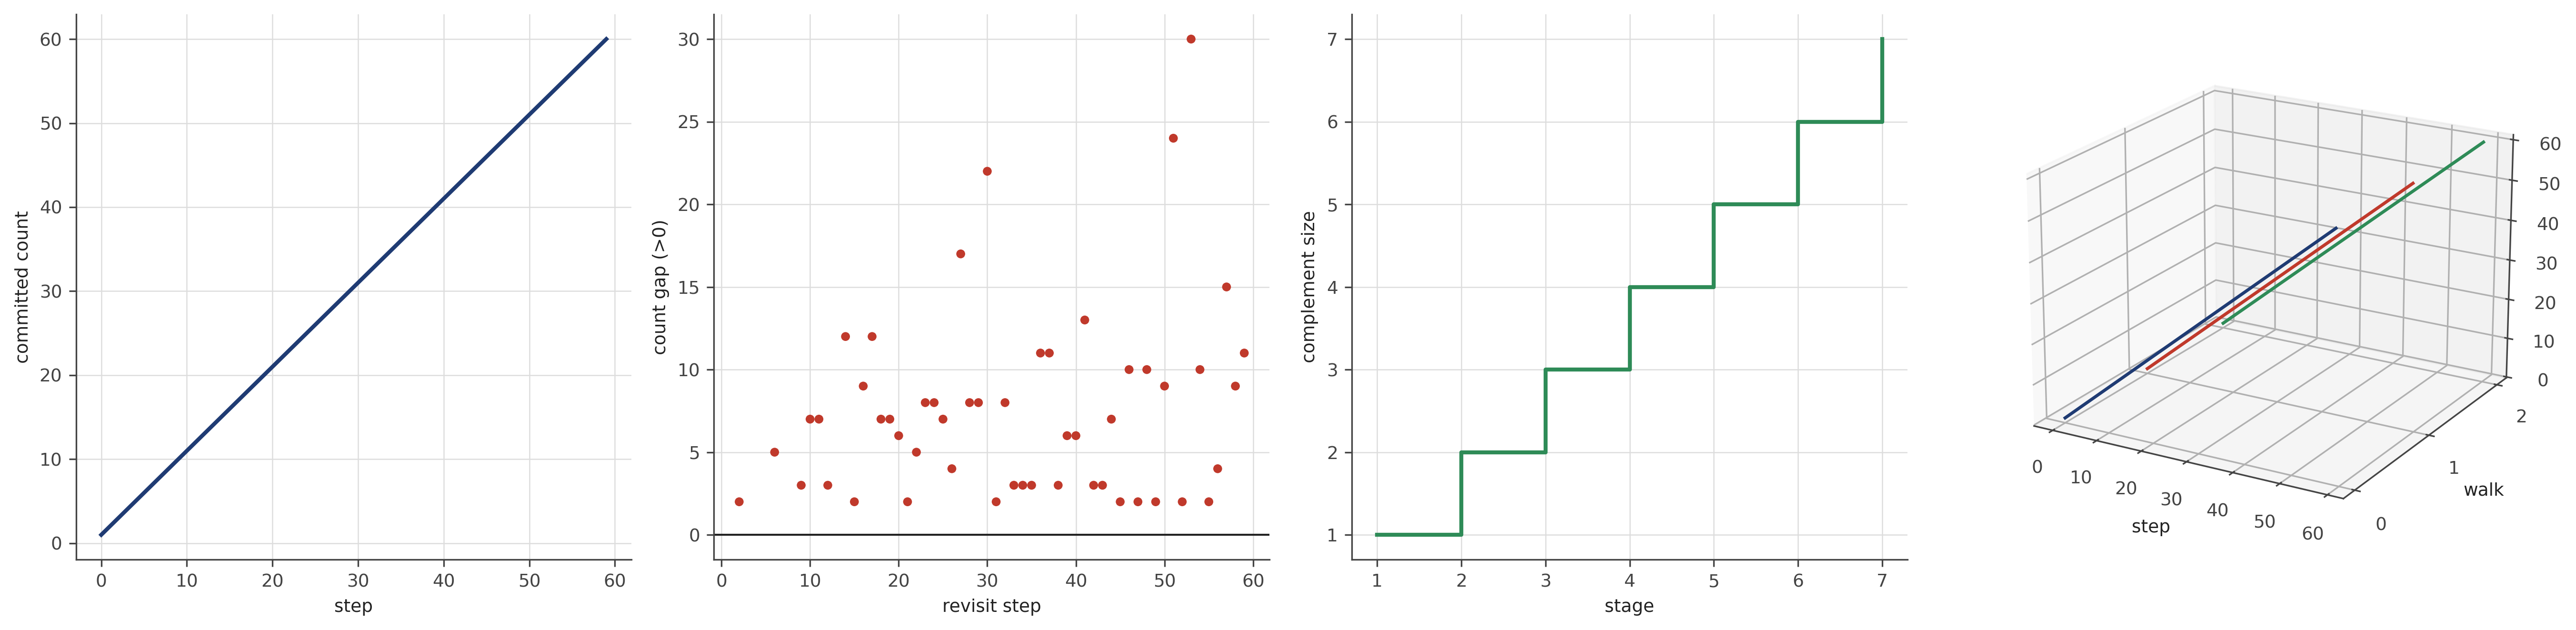
\includegraphics[width=\textwidth]{figures/panel_7.png}
    \caption{\textbf{T6, histories do not return.}
    (\textbf{A})~Committed count versus step along a gated walk: strictly
    increasing (\Cref{thm:nonreturn}).
    (\textbf{B})~At every revisit of a vertex, the count gap to its previous visit
    is strictly positive (all points above the line at $0$): revisiting is not
    returning.
    (\textbf{C})~The complement of a fixed part grows monotonically with the stage
    of a progressing whole (\Cref{thm:temporal-nonreturn}): a thing is
    distinguishable from its earlier stage.
    (\textbf{D})~Three independent gated walks, committed count versus step,
    all strictly monotone. Viewing angle: elevation $20^{\circ}$, azimuth
    $-60^{\circ}$.}
    \label{fig:panel-T6}
\end{figure*}

\begin{figure*}[!htbp]
    \centering
    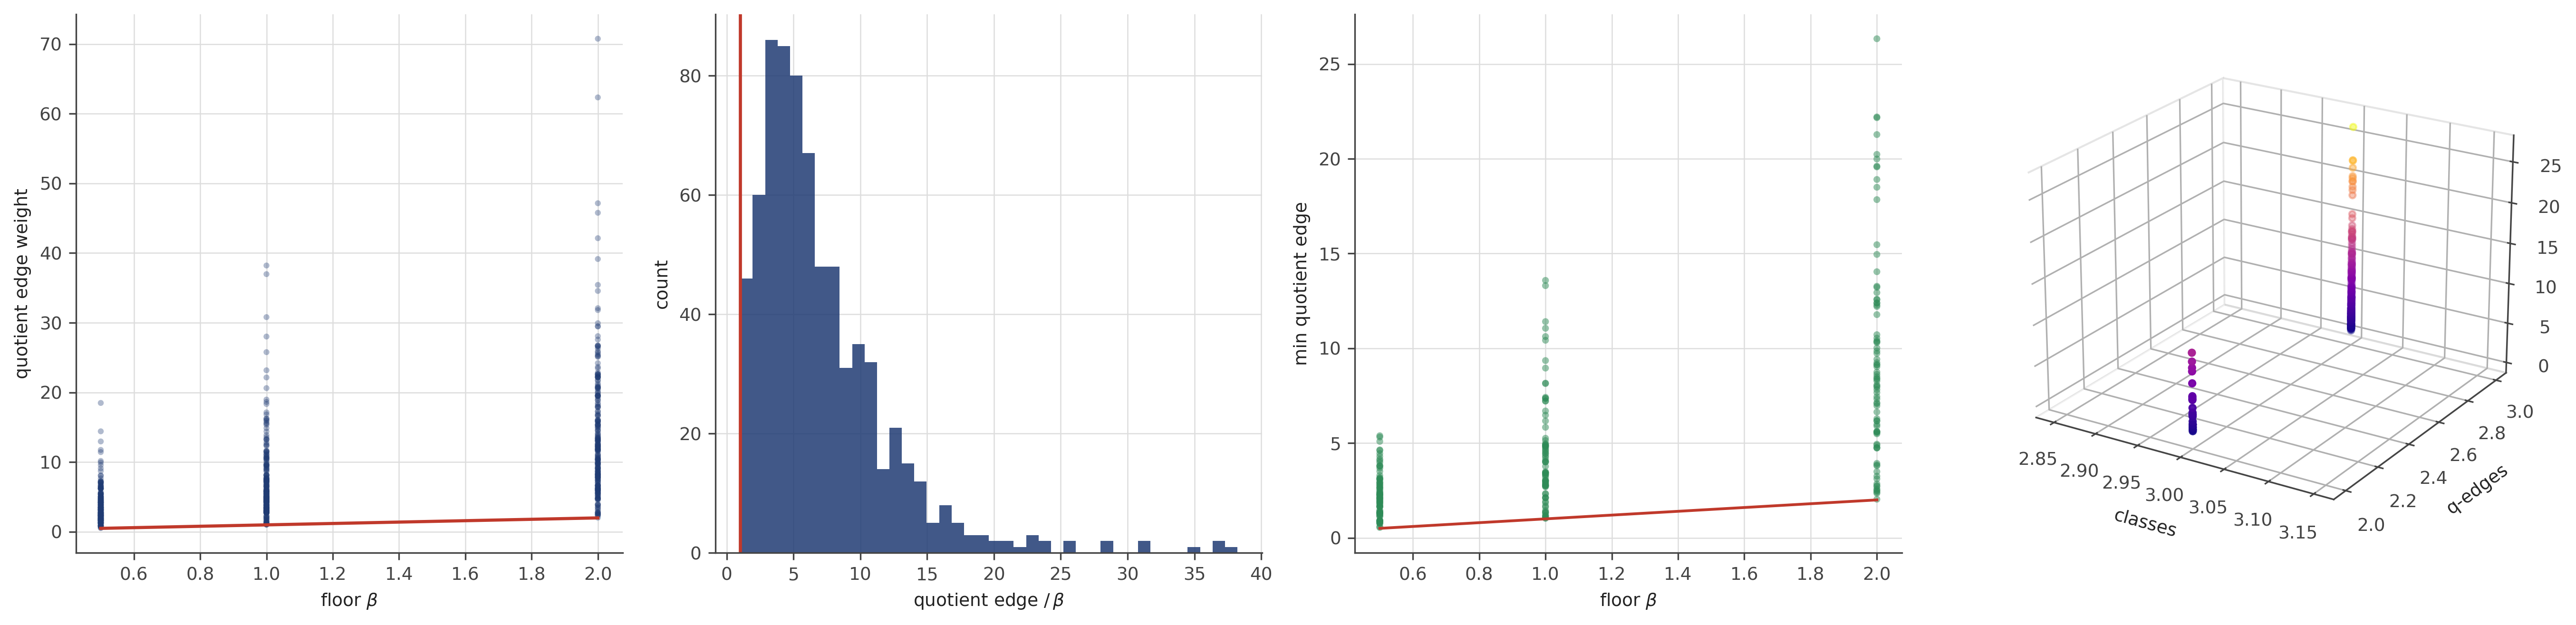
\includegraphics[width=\textwidth]{figures/panel_8.png}
    \caption{\textbf{T7, the quotient inherits a floor.}
    (\textbf{A})~Quotient edge weight (a class-to-class cut) versus floor, on or
    above $y=\beta$ (red): the collective is again a contact graph
    (\Cref{lem:quotient-floor}).
    (\textbf{B})~Distribution of quotient-edge$/\beta$, supported above $1$ (red).
    (\textbf{C})~Per-instance minimum quotient edge versus floor, above the
    equality line.
    (\textbf{D})~Three-dimensional surface of the minimum quotient edge over class
    count and quotient-edge count. Viewing angle: elevation $22^{\circ}$, azimuth
    $-58^{\circ}$.}
    \label{fig:panel-T7}
\end{figure*}

\subsection{Authored structures and measurement}

\begin{figure*}[!htbp]
    \centering
    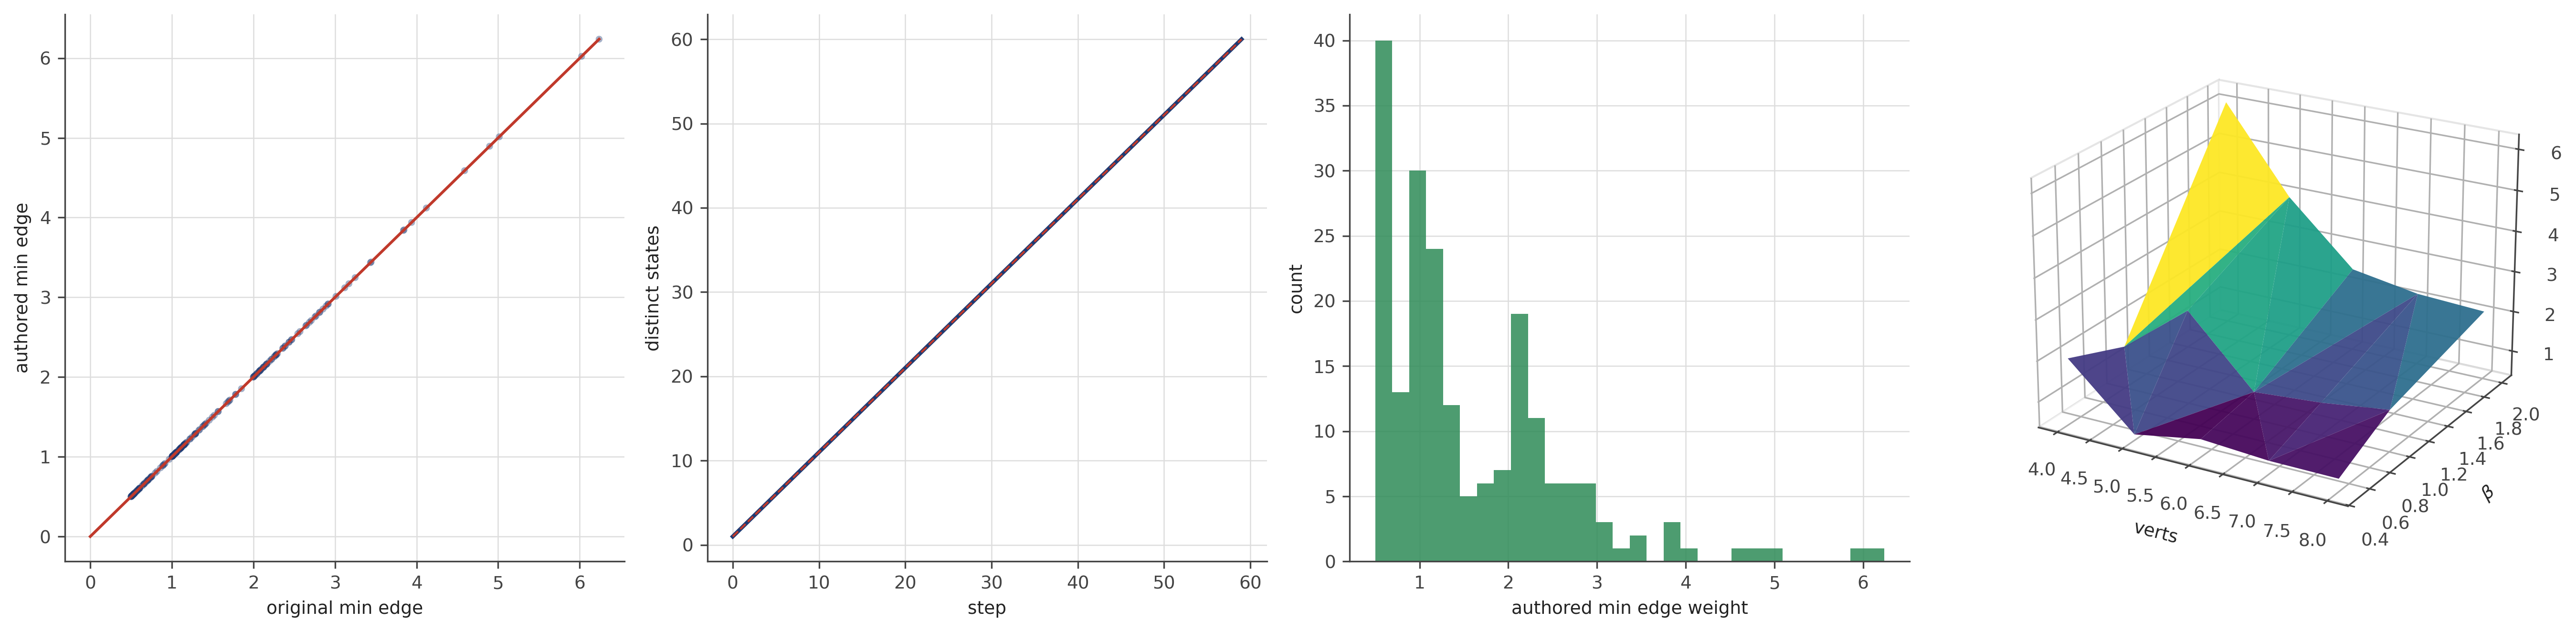
\includegraphics[width=\textwidth]{figures/panel_9.png}
    \caption{\textbf{T8, authored structures exist and are bounded.}
    (\textbf{A})~Minimum edge weight of an authored instance versus that of the
    original, on the diagonal: specify-then-instantiate preserves the floor
    (\Cref{thm:authored-exist}).
    (\textbf{B})~Distinct states of an authored structure's forward closure versus
    step, tracking the line of slope one (grey dashed): every state is new
    (open-endedness, \Cref{thm:open}).
    (\textbf{C})~Distribution of authored minimum edge weight, bounded below by the
    floor (floor-limited authorship, \Cref{thm:floor-limited}).
    (\textbf{D})~Three-dimensional surface of the authored minimum edge over vertex
    count and floor, never sub-floor. Viewing angle: elevation $22^{\circ}$,
    azimuth $-60^{\circ}$.}
    \label{fig:panel-T8}
\end{figure*}

\begin{figure*}[!htbp]
    \centering
    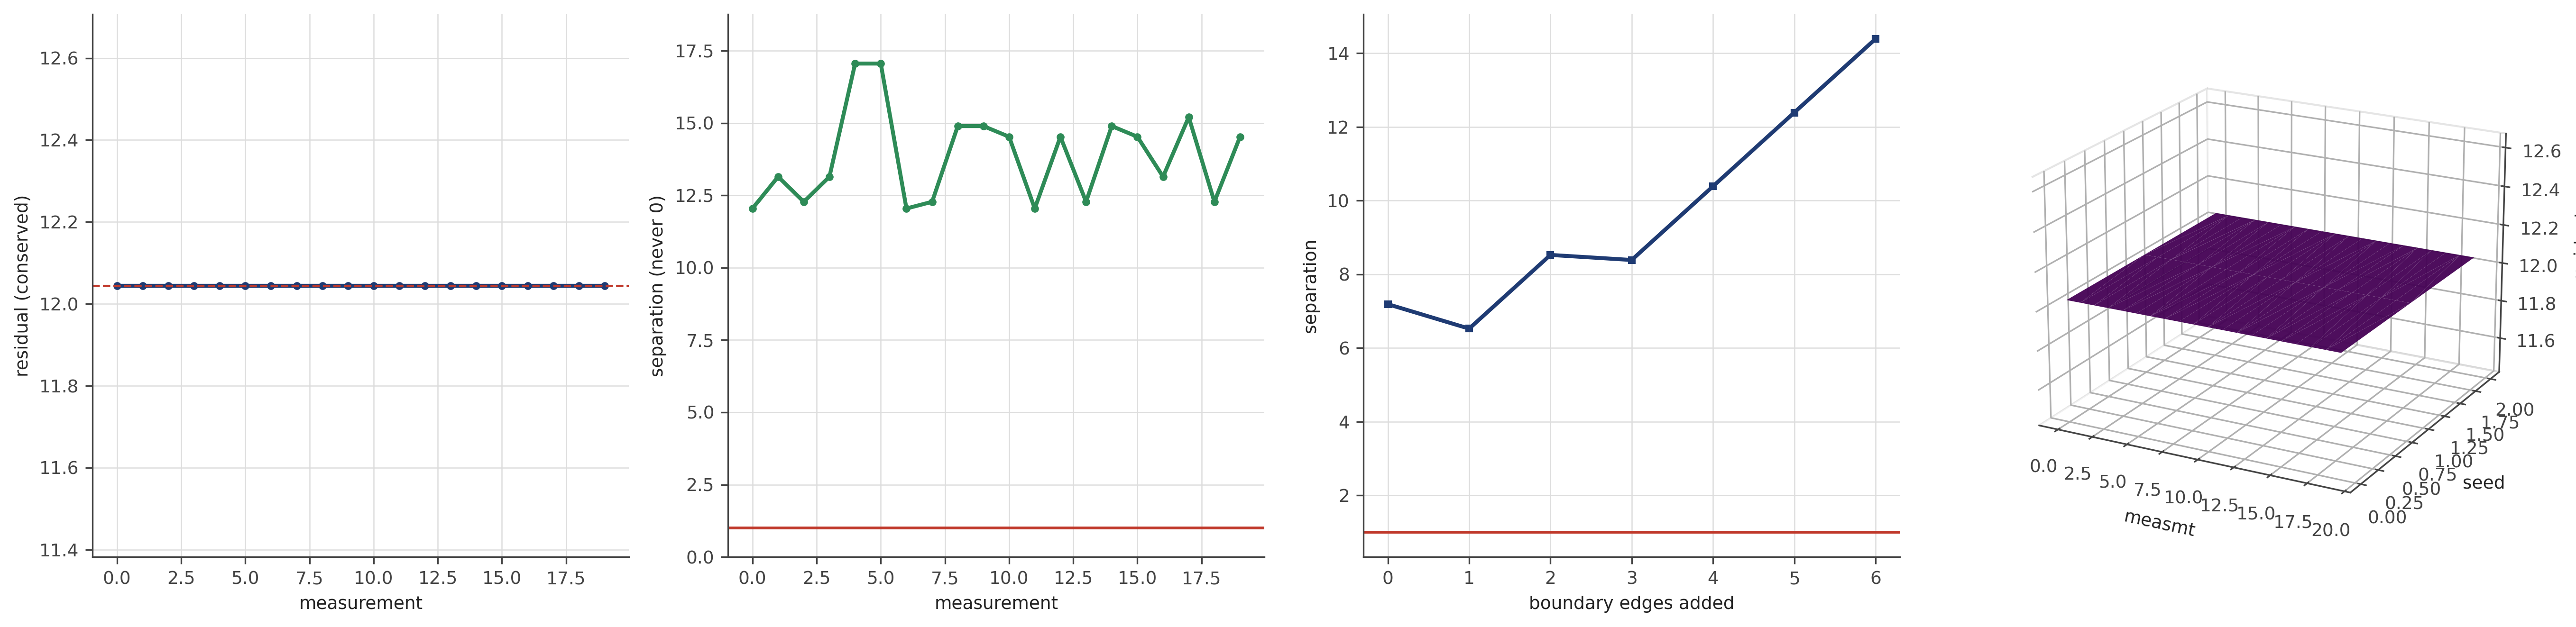
\includegraphics[width=\textwidth]{figures/panel_10.png}
    \caption{\textbf{Measurement: the invariant is conserved and identity is
    unreachable.}
    (\textbf{A})~Residual across $20$ successive measurements (reshufflings): a
    flat line at its initial value (red dashed)---measurement conserves the
    invariant (\Cref{prop:measure-conserves}).
    (\textbf{B})~Separation of a fixed part from the medium across measurements:
    it fluctuates but never falls to the floor line (red) and never reaches zero
    (self-defeat, \Cref{thm:self-defeat}): identity is not resolved to a point.
    (\textbf{C})~Separation versus the number of boundary edges added: it rises and
    never collapses, staying above the floor (red)---resolution does not saturate
    (\Cref{prop:resolution}).
    (\textbf{D})~Three-dimensional surface of the residual over measurement index
    and three independent reshuffling seeds: a flat plane---conserved on every
    seed. Viewing angle: elevation $20^{\circ}$, azimuth $-62^{\circ}$.}
    \label{fig:panel-measurement}
\end{figure*}

\begin{remark}[Status of the numerical witness]
\label{rem:numerical-status}
The figures confirm the results on concrete instances and display their
quantitative form; they are evidence of correctness and magnitude, not a
substitute for the proofs, which hold for every contact graph satisfying
\Cref{ax:finite} in a non-completable whole. That all $149{,}793$ checks across
$600$ independently constructed instances agreed with the predicted bounds---no
sharp cut, the residual conserved under every reshuffling, the separation never
reaching zero---is consistent with the claim that the floor is structural and
that identity, the conserved interior, is unreachable by measurement.
\end{remark}
